\chapter{Vortex analysis of two-dimensional superfluid systems}
\label{ch:2d}

Here, we show an application of the GPUE codebase in simulating a two-dimensional chaotic system with few vortices.
This chapter makes heavy use of the vortex tracking, rotation, and phase-imprinting methods described in Chapter~\ref{ch:gpu}.
In addition, this chapter intends to display the dependence of post-processing metrics to dynamical studies of superfluid systems.

In a similar fashion to Chapter~\ref{ch:1d}, this chapter will start with a disclaimer about the dimensionality of the systems we will be simulating.
In principle, all real-world physics is three-dimensional, but in a similar fashion to how a one dimensional cigar-shaped BEC can be created, a pancake-like geometry can also be constructed by increasing the trapping frequency in the $\hat z$ (perpendicular) direction with respect to the $\hat x$ and $\hat y$ (transverse) directions.
With this geometry, we can assume that the condensate is in the ground state along the $\hat z$ dimension and rewrite the wavefunction as $\Psi(\mathbf{r},t) = \Psi(x, y, t)\phi(z)$, where $\Psi(x, y, t)$ is the wavefunction in the transverse plane and $\phi(z) = (m \omega_z/(\pi\hbar))\text{exp}(z^2 m\omega_z/(2\hbar))$ is the ground state along the $\hat z$ dimension.
By integrating over $\hat z$, we also find that the interaction strength is modified for a two-dimensional consensate to be

\begin{equation}
g_{2D} = g \sqrt{\frac{m\omega_z}{2\pi\hbar}}.
\end{equation}

\noindent With these changes, we can simulate two-dimensional quantum simulations with the GPUE codebase~\cite{zhang2019, o2017, o2016topo, o2016}.

This chapter will apply several of the techniques mentioned in Chapters~\ref{ch:splitop} and \ref{ch:gpu} to a rotating two-dimensional BEC system for a small number of vortices and will follow the work of Zhang \textit{et.al.}~\cite{zhang2019}.

\section{Chaotic few-body vortex dynamics in rotating Bose--Einstein condensates}

Chaotic evolution is typically identified by a significant divergence in trajectory based on a small change in the initial conditions~\cite{strogatz2018}, and it is possible to find such an environment in turbulent flows~\cite{spiegel1987, biferale2005}.
For classically turbulent flow, the degree of chaos depends on the Reynolds number~\cite{berera2018}; however, the nature of quantum turbulent effects is still an active area of research~\cite{white2014}.
Because superfluid vortices are relatively simple compared to their classical counterparts, there has also been significant interest in the differences between classical and quantum turbulence~\cite{nemirovskii1995,kyriakopoulos2014,koukouloyannis2014,navarro2013}.
In spite of the differences between the fluid models, vortex dynamics in superfluid systems are remarkably similar to classical point-vortex models and key features of classical turbulence, such as the Kolmogorov spectrum have been shown to exist for large, turbulent, quantum systems~\cite{nore1997,stalp1999,araki2002,salort2010}.

In this study, we would like to create a quantum system that is chaotic without relying on quantum turbulence, and
it is known that it is not possible to excite quantum chaos in large vortex lattices, as these systems have been proven to be stable to external perturbations~\cite{o2017}.
For this reason, we wish to probe quantum chaos with a small number of vortices, such that quantum tuburlent effects are not excited.
These chaotic, few-vortex systems have been studied previously by Aref and Pomphrey~\cite{aref1982, aref1980, aref1983}, who showed that quantum chaos can be excited in systems with as few as four vortices in an infinite plane~\cite{aref1982}.
Unlike classical chaos, the onset of quantum chaos seems to appear with fewer vortices present, and few-vortex systems have been explored experimentally for two, three, and four vortices in harmonically trapped BECs~\cite{navarro2013}.
When analyzed with a reduced Hamiltonian approach, harmonically trapped BECs seem exhibit chaotic effects with as few as three vortices, two co-rotating vortices and an anti-vortex rotating in the other direction~\cite{kyriakopoulos2014,koukouloyannis2014}.

Experimentally, it is now possible to detect vortex circulation~\cite{seo2017}, image vortices in-situ~\cite{wilson2015}, and probe vortex dynamics at different times within a single experiment~\cite{freilich2010, serafini2017}.
Because quantum vortices are simple and BECs are highly controllable experimental systems in two-dimensions, there has been significant interest in two-dimensional quantum turbulent systems as well~\cite{neely2013,shin2004}.
Additional effects, such as the K\'arm\'an vortex street~\cite{kwon2014} and Onsager vortex clusters~\cite{gauthier2018,johnstone2018} have also been shown to exist experimentally.

In order to engineer well-controlled initial conditions, we will create a small vortex lattice of four vortices, and then create a small defect via phase imprinting.
This process will controllably induce chaotic vortex dynamics in an experimentally feasible way.
We also show that these chaotic dynamics are enhanced by the close approach of vortices in the simulated results.
By using phase imprinting in this way on a larger number of vortices in a vortex lattice, it might be possible to induce chaotic events there as well, which might enable studying a set of vortex trajectories that is chaotic at specific points, but stable overall.

\section{Model}

\begin{figure}
\center 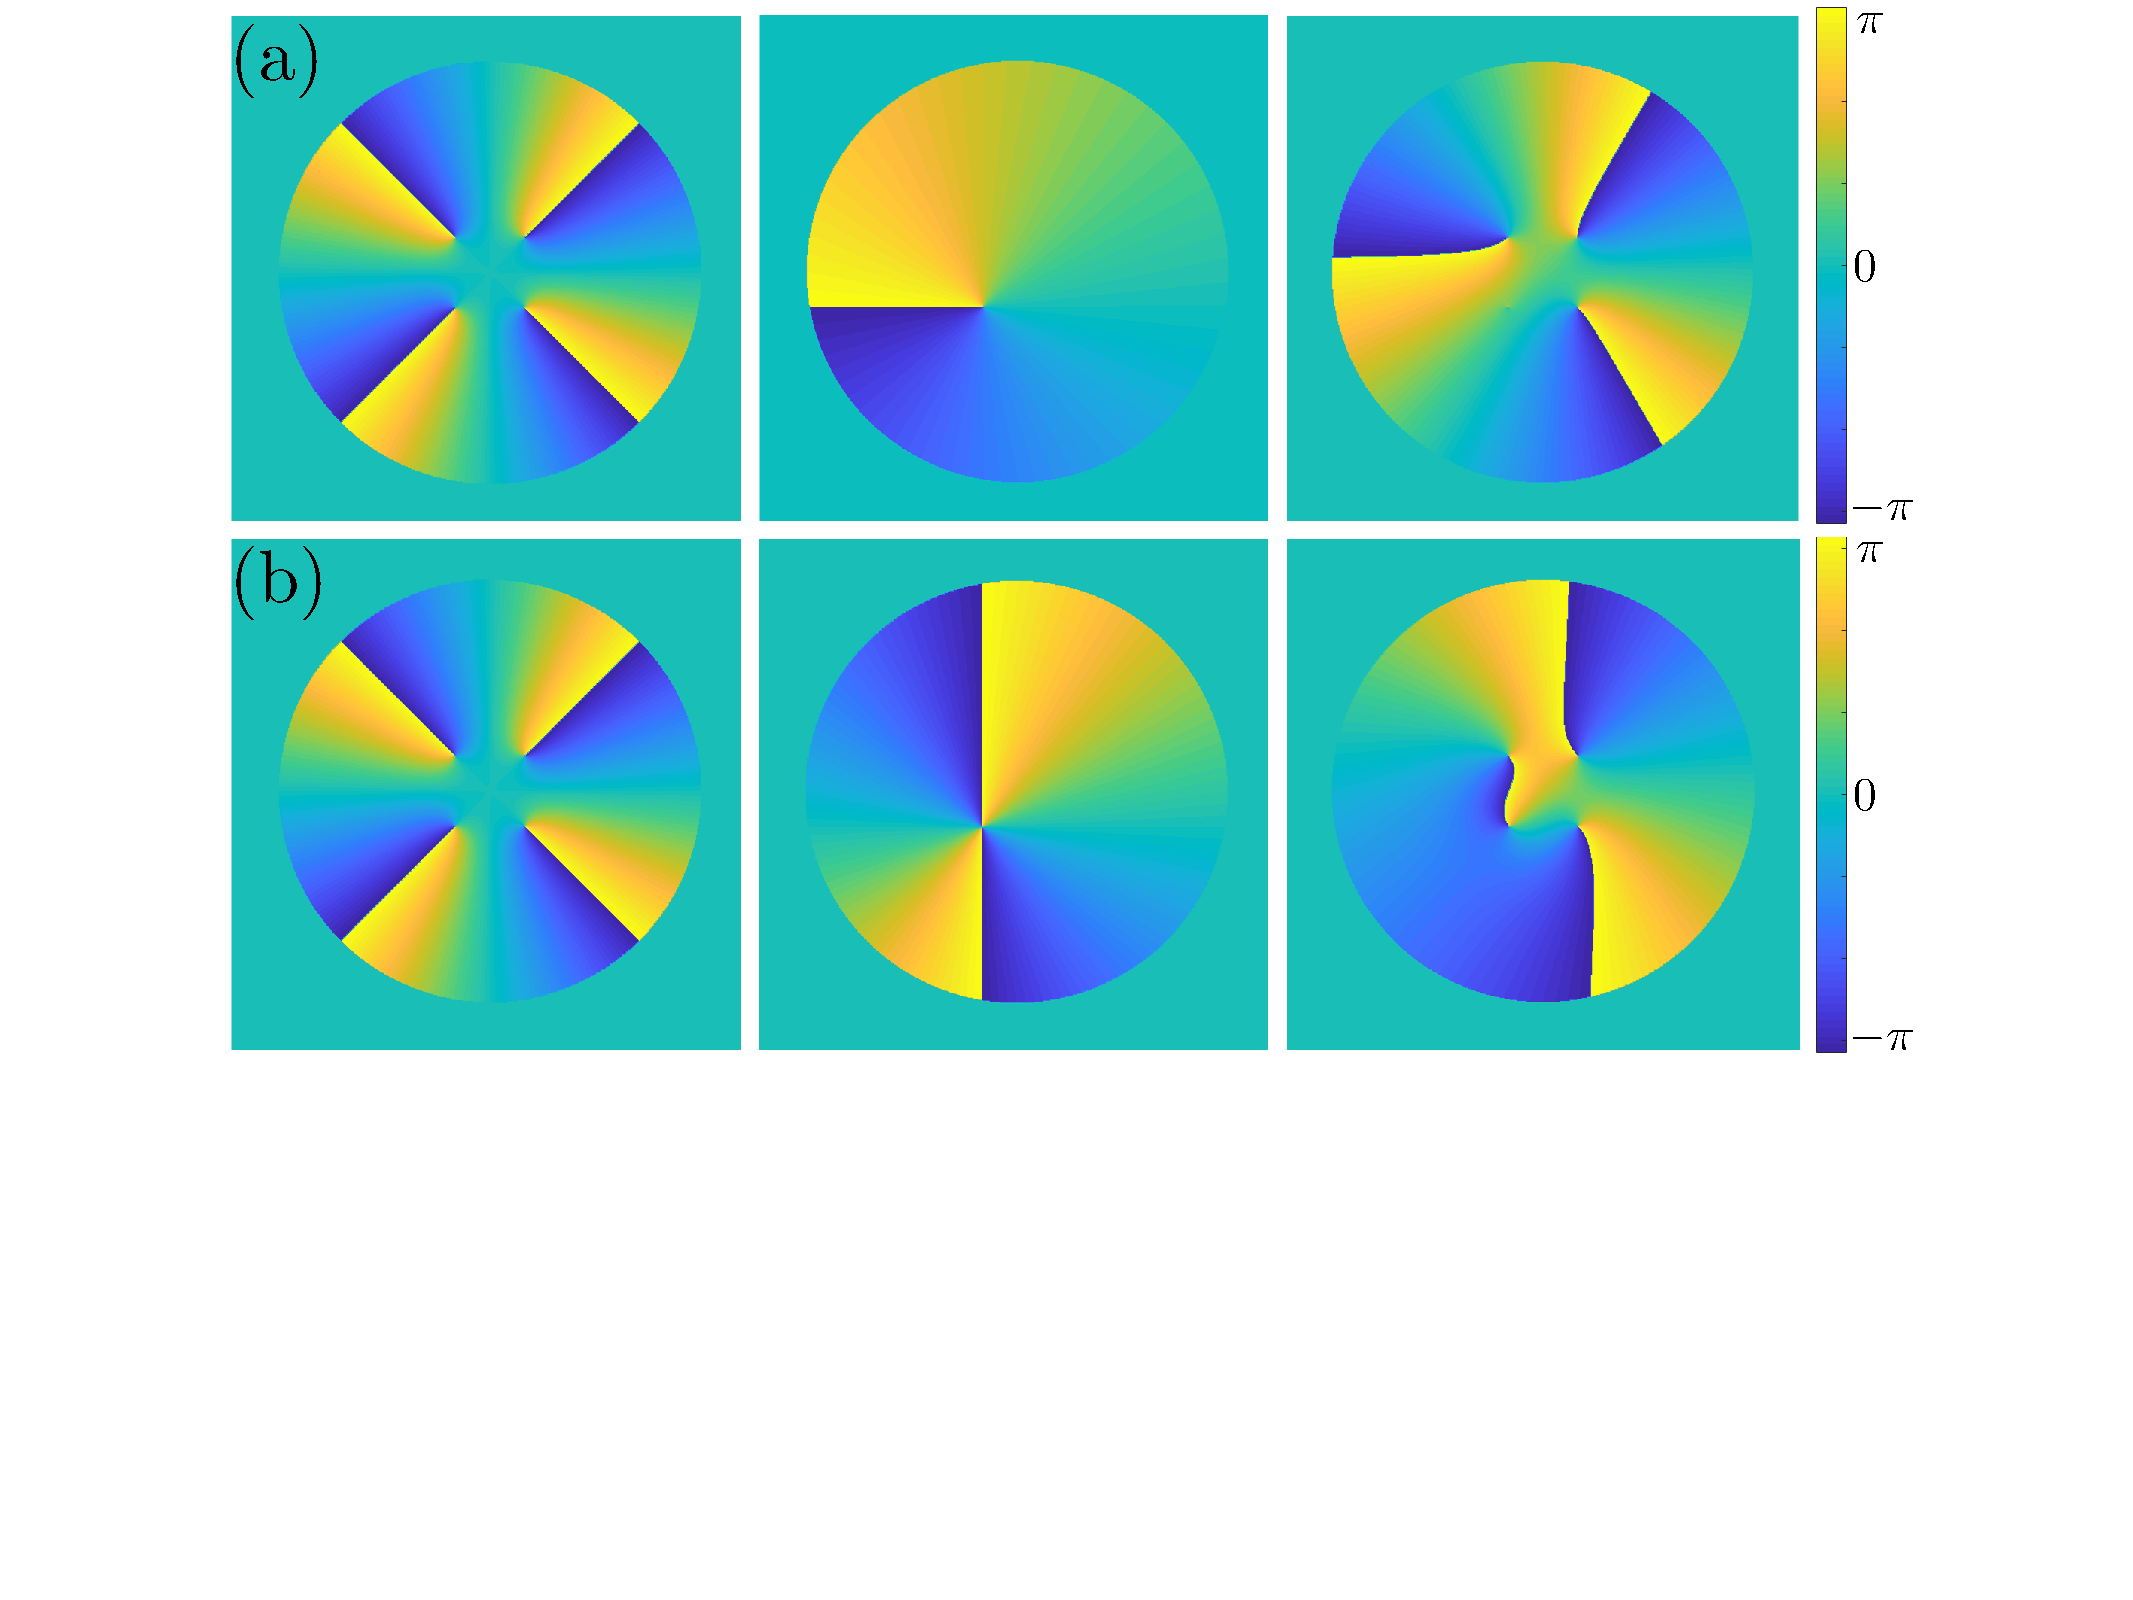
\includegraphics[width=0.75\textwidth]{data/2d/phase/phase}

\caption{
The initial four co-rotating vortex system is shown at the left.
In the center is the applied phase mask of $-2\pi$ for (a) and $-4\pi$ for (b), and the resulting phase distribution is shown on the right.
Here we see that by applying a $-2\pi$ phase winding, we erase a vortex from the system, and by applying a $-4\pi$ phase winding, we flip the vortex, creating an anti-vortex.
}
\label{fig:phase}
\end{figure}


For this study, we created a condensate with $N = 10^6$ $^{87}$Rb atoms with an s-wave scattering length of $a_s \approx 90a_0$ in a pancake geometry with typical trapping frequencies of $(\omega_\perp, \omega_z) = (2\pi, 32\pi)$Hz.
Here, the s-wave scattering length is $a_s \approx 90a_0$ and the effective interaction strength is $g = 6.8\times 10^{-40}$ m$^4$kg/s$^2$.
These simulations were performed on a grid of $2^{10} \times 2^{1-}$ points and covering an extent of $700\mu \text{m} \times 700 \mu \text{m}$

First, ground-state evolution was performed with a low rotation frequency of $\Omega = 0.3 \times 2\pi$ Hz via GPUE~\cite{schloss2018}.
Though large rotational frequencies will create a triangular lattice, for smaller frequencies, other configurations are known ~\cite{aftalion2001}, and we will focus on the regine where the ground state is composed of four vortices in a square configuration~\cite{zampetaki2013}.
Once this configuration is achieved, we then manipulate a vortex via phase imprinting, such that three co-rotating vortices and one anti-vortex exist in the system.
Examples of phase imprinting on this system can be seen in figure~\ref{fig:phase}, where the top row shows a simple vortex annihilation and the bottom row shows a vortex flip.

\section{Regular and irregular vortex dynamics}

\begin{figure}
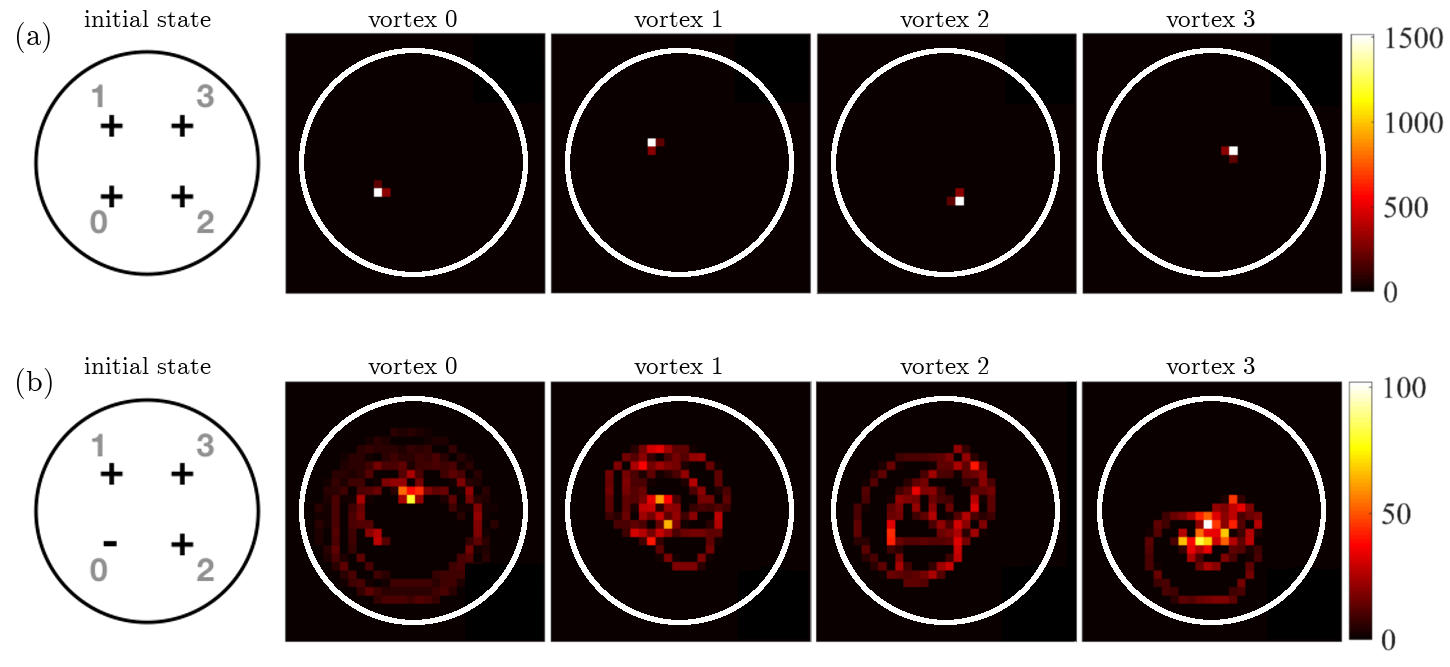
\includegraphics[width=\textwidth]{data/2d/histogram/histogram}

\caption{
Histograms of the positions of each vortex in the transversal plane for 20 secons in the co-rotating frame.
The lower left vortex has been annihilated and re-imprinted with (a) the same and (b) the opposite direction of rotation, exactly on the location of the previous vortex.
The area of each plot is $400\mu \text(m) \times 400 \mu \text{m}$, and the white circles correspond to iso-lines at 40\% the maximum density to highlight the extent of the vortex motion.
In (a), we see that if all four vortices are co-rotating, regular trajectories appear, but in (b), we see that flipping the rotation direction of a single vortex creates disordered trajectories.
}
\label{fig:histogram}
\end{figure}

It is known that a lattice of vortices with the same direction of rotation will exhibit regular dymanics~\cite{abo2001}, and in Figure~\ref{fig:histogram}(a), we confirm this for a system of four vortices.
In this figure, we show a histogram of the vortex trajectory over 20 seconds of evolution when removing and then re-imprinting a vortex of the same rotational direction at the same location
Even though a small residual movement appears due to small phonon excitations that were not fully removed from the imaginary time evolution, the vortices remain stationary.
In Figure~\ref{fig:histogram}(b), we also show that if the re-imprinted rotation is of the opposite direction, the vortex dynamics become more disordered, with vortices traversing a larger width of the condensate.
It is worth mentioning that these histograms can be constructed experimentally with available imaging techniques~\cite{wilson2015,freilich2010}.

\begin{figure}
\center 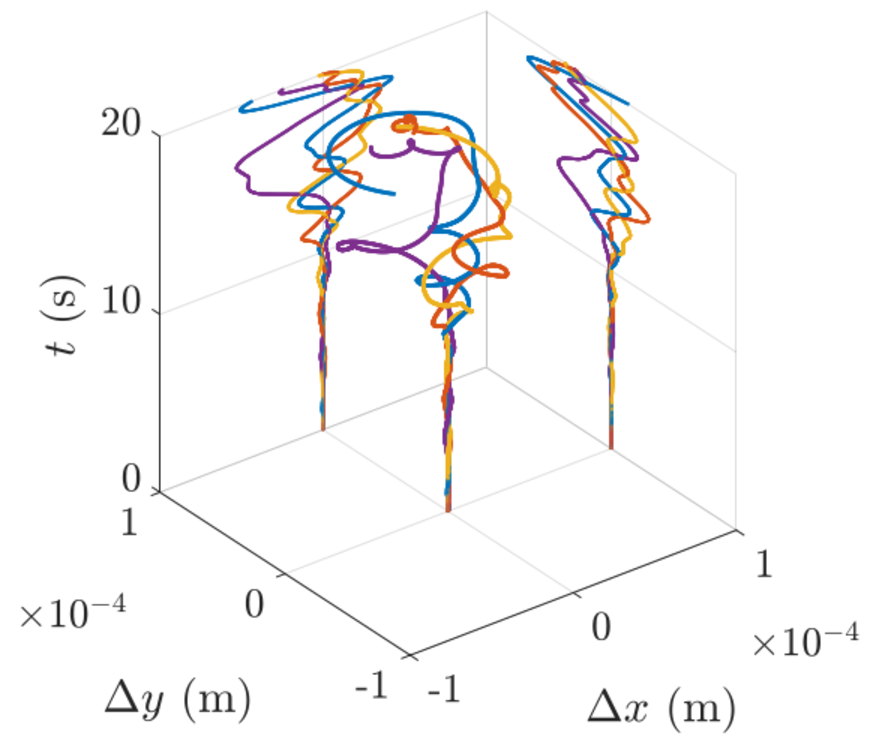
\includegraphics[width=0.5\textwidth]{data/2d/evolution/evolution}

\caption{
Evolution of the difference in trajectories $\triangle \textbf{r}_i = \textbf{r}_{i}-\textbf{r}'_{i}$ with $\textbf{r}$ corresponding to the position of the $i$th vortex from the center of the condensate and $i\in \{0,\ 1,\ 2,\ 3\}$ labelling each individual vortex for the four-vortex system as shown in Fig.~\ref{fig:histogram}.
A small change in the initial position of the anti-vortex arises from a phase-imprint at $(x_{0},y_{0})$ and $(x_{0}-\xi/3,y_{0})$ where $(x_{0},y_{0})$ denotes the pre-existing co-rotating vortex core position.
The curves show that even though the onset of disorder is immediate, a strong divergence of trajectories is observed at about $t\approx 10 \text{s}$ (see projections onto the $x$-$t$ and $y$-$t$ planes).
The difference in trajectory of the anti-vortex, $\Delta \mathbf{r}_0$, is shown in blue, while yellow, orange, and purple lines depict the three co-rotating vortices.
}
\label{fig:evolution}
\end{figure}

Even though the introduction of the anti-vortex creates a disordered trajectory, it could be entirely possible that this trajectory is stable.
To uniquely identify chaotic behaviour, we need to show that any small perterbation in the vortex location will also provide a significantly different trajectory.
To check this, we compare two sets of vortex trajectories with slightly different shifts in the initial position of the anti-vortex, $\mathbf{r}_0$ and $\mathbf{r}'_0$, where $\mathbf{r}_0 - \mathbf{r}'_0 = \xi/3$ and $\xi$ is the healing length.
In Figure~\ref{fig:evolution}, we show the differences in trajectories, defined as $\Delta \mathbf{r}_i(t) = \mathbf{r}_{i}(t)-\mathbf{r}'_{i}(t)$ in Figure.~\ref{fig:histogram}, where $\mathbf{r}$ refers to the position of the $i$th vortex from the center of the condensate and $i\in \{1,2,3\}$ corresponds to the vortex number.
Here, we see that the difference in trajectory is initially small, but diverges significantly at around $t \approx 10$ seconds, which is a strong indication of chaotic behavior.

After closely inspecting the vortex dynamics (shown in the supplementary movie~\ref{movie}), we see that this strong divergence in vortex trajectories seems to be accelerated when all four vortices come in close proximity.
Because the velocity fields of each vortex decays as $1/\mathbf{r}$, where $\mathbf{r}$ is the distance from the core, the vortices experience stronger velocity fields when they are closer; therefore, the point of minimal separation can be seen as a highly nonlinear multi-vortex scattering event that accelerates the divergence shown in Figure~\ref{fig:evolution}.
In Figure~\ref{fig:snapshots} we study this further by showing snapshots of the condensate density before ($t = 6$s), at ($t = 10$s), and after ($t = 15$s) the scattering event are shown in (a) and (b) for the non-shifted and shifted anti-vortex locations.
The differences between position of each vortex and the anti-vortex is also shown (b) for the case where the anti-vortex is shifted by $\xi/3$.
Here, we see that there is a clear minimum at $t \approx 10$s, which is the same time at which the  trajetories begin to diverge in Figure~\ref{fig:evolution}
In order to characterize this divergence in trajectory, we must analyze the vortex dynamics in more detail and calculate the Lyapunov exponent

\begin{figure}
\center 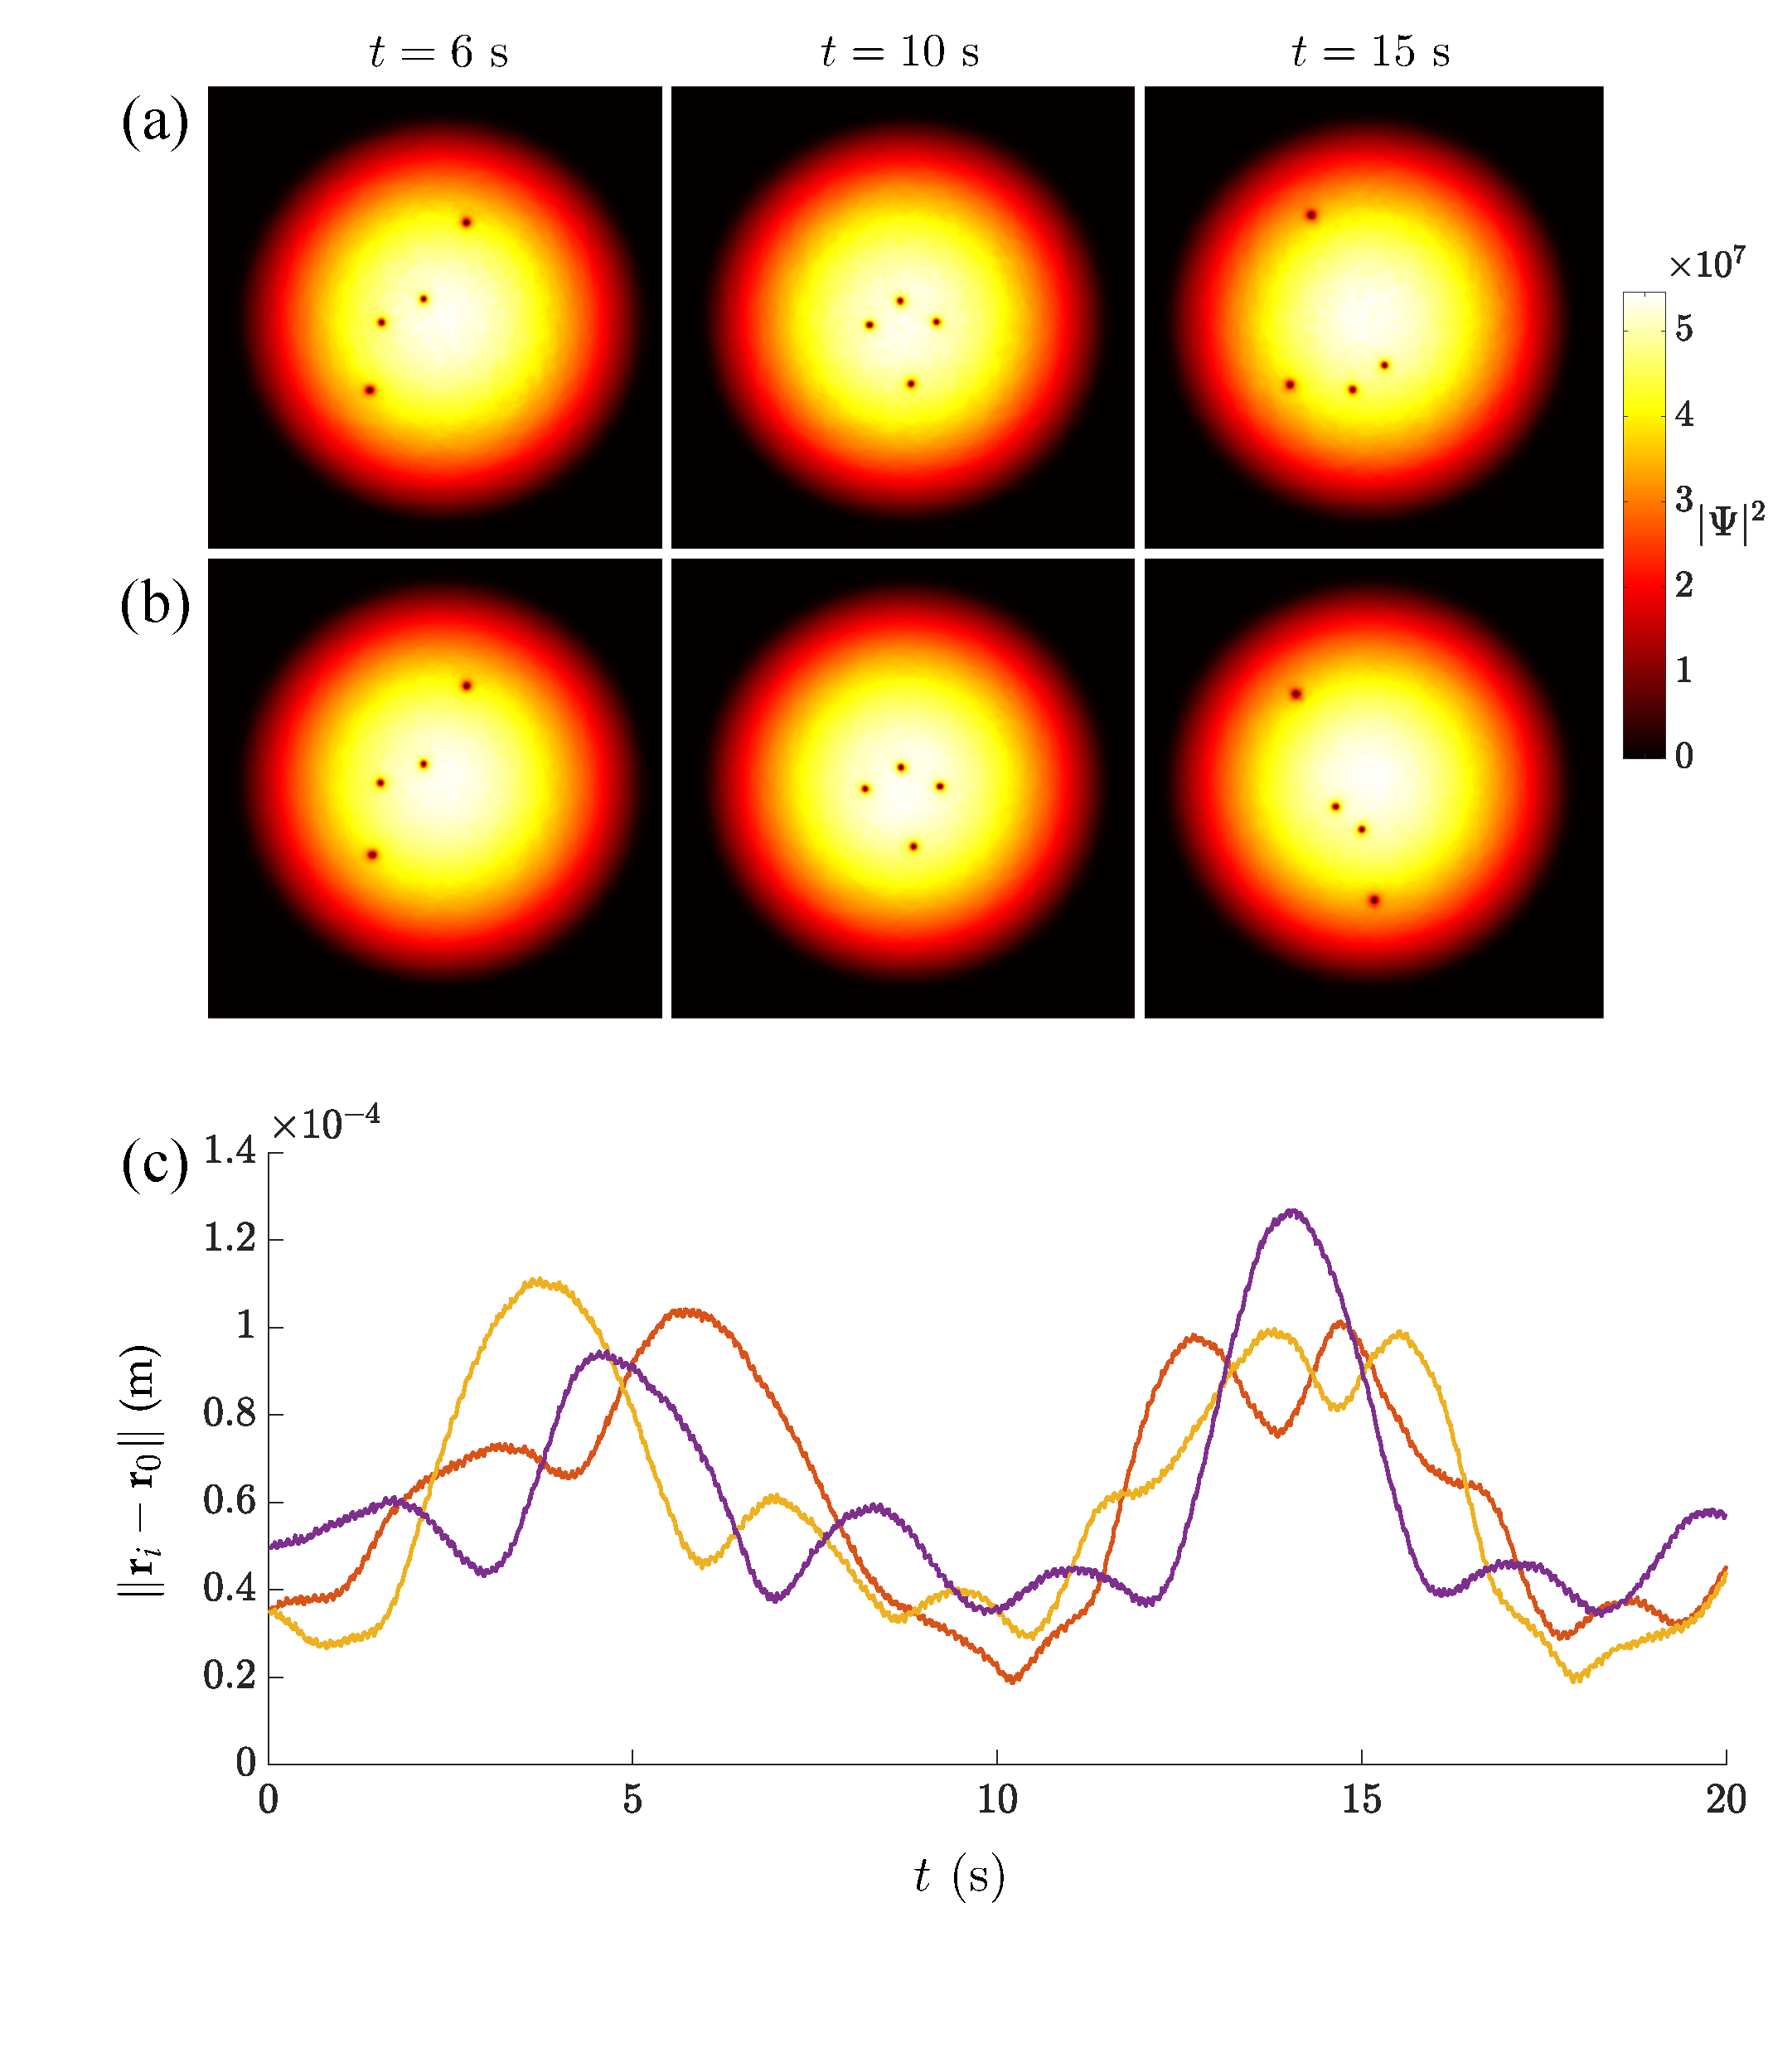
\includegraphics[width=0.75\textwidth]{data/2d/snapshots/snapshots}

\caption{
Density plots of condensate for (a) $\Delta x = 0$ and (b)$\Delta x=\xi/3$ at times $t=\{6,10,15\}$ s. The densities before the scattering event differ only on small scales (see $t=6s$), whereas for times after the event large deviations are visible (see $t=15s$).
At $t=10s$ the vortices make their closest approach. The area plotted is $500 \mu m\times 500 \mu m$.
(c) Distances between the vortices at positions $\mathbf{r}_i$ with $\mathbf{r}$ corresponding to the position of the $i$th vortex from the center of the condensate and $i\in \{1,2,3\}$ corresponding to the vortex number as shown in Fig.~\ref{fig:histogram} and anti-vortex at $\mathbf{r}_0$ for $\Delta x = 0$.
A minimum around $t=10s$ is clearly visible.
}
\label{fig:snapshots}
\end{figure}

\section{Characterizing chaotic vortex dynamics}

\begin{figure}
\center 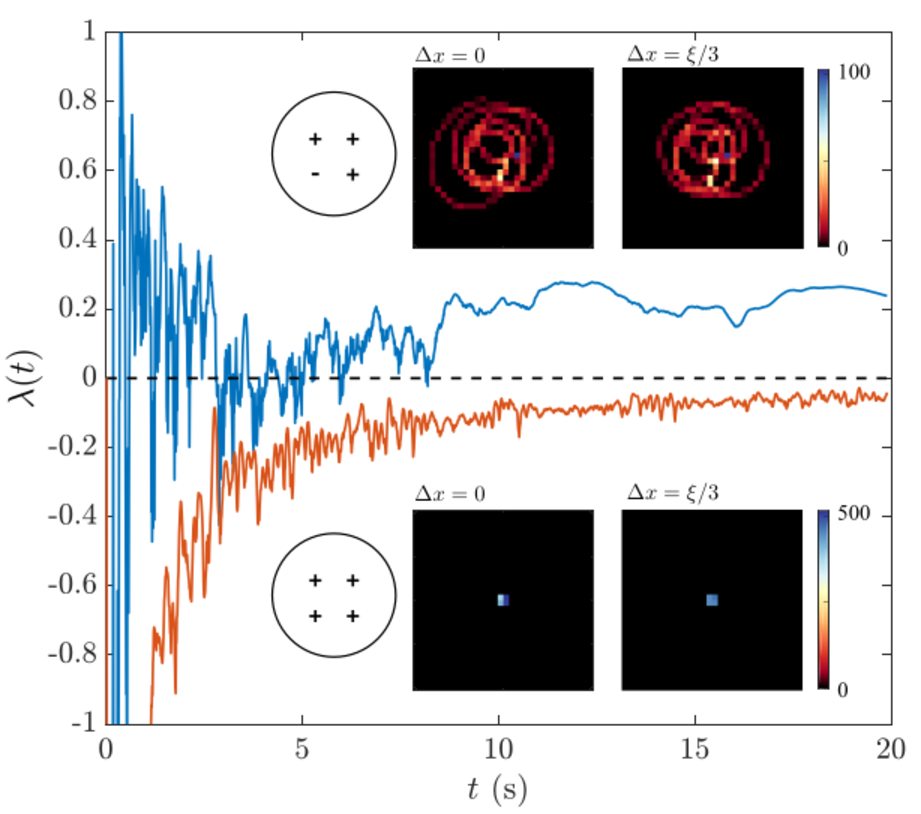
\includegraphics[width=0.75\textwidth]{data/2d/lyap/lyap}

\caption{
The insets show the histograms of the COM trajectories calculated over 20 seconds of evolution for the system of four vortices when the position of a single vortex has been shifted by $\Delta x=0\xi$ and $\Delta x=\xi/3$.
The upper two panels depict the corresponding trajectories after the direction of rotation of a single vortex has been reversed, whereas the lower row displays the trajectories for the case where all vortices co-rotate.
The main curve plots the corresponding Lyapunov exponents,  calculated from the shown COM trajectories. 
The negative Lyapunov exponents (orange) indicate that shifting the vortex about the initial position still ensures the stability of vortex trajectories. Reversing the direction of circulation of a single vortex (blue) however leads to fluctuations about zero, eventually leading to a fully positive exponent. 
}
\label{fig:lyap}
\end{figure}


To characterize the degree of chaos for the shown vortex dynamics, we have chosen to use Lyapunov exponents, which give the rates of divergence for nearby orbits in phase space~\cite{wolf1985}.
With this measure, we track two trajectories in phase space and assume that the divergence between the two trajectories will either exponentially converge or diverge, and we can model this behaviour with

\begin{equation}
|\delta\mathbf{Z}(t)| \approx e^{\lambda t} |\delta \mathbf{Z}_0|.
\end{equation}

\noindent Here, $\delta\mathbf{Z}_0$ is the initial separation between the trajectories and $\lambda$ is a quantity known as the Lyapunov exponent.
If the exponent is negative, it means that the trajectories tend to converge, but it it is positive, the trajectories will diverge, thus indicating chaotic motion.
The rate of divergence is determined by the value of the exponent.

For out simulation, we model the trajectories in four-dimensional phase-space with $\mathbf{P(t)} = (x(t), y(t), v_x(t), v_y(t))$ and $\mathbf{P}'(t) = (x'(t), y'(t), v'_x(t), v'_y(t))$.
The separation is then defined to be $\delta \mathbf{P(t)} = (\delta x(t), \delta y(t), \delta v_x(t), \delta v_y(t))$ where $\delta x(t) = x(t) - x'(t)$, etc.
The exponent can then be calculated as

\begin{equation}
\lambda = \lim_{t\to\infty}\frac{1}{t}\text{ln}\frac{||\delta\textbf{P}(t)||}{||\delta\textbf{P}(0)||}
\label{eqn:lyap}
\end{equation}

\noindent where $||\cdot||$ denotes the Euclidean norm.

In this case, we track each vortex with the methods outlined in Chapter~\ref{ch:gpu}, and use both the position and velocity of the vortex.
Because we wish to determine whether the total system is chaotic, beyond its constituent vortices, we use a center of mass (COM) variable, defined as $\mathbf{R}_M = \frac{1}{n+1}\sum_{i=0}^nr_i$, where $n+1$ is the number of vortices.
Similarly, the center of velocity is defined as $\mathbf{v}_M = \frac{1}{n+1}\sum_{i=0}^nv_i$.
These values are then used with Equation~\ref{eqn:lyap}, and the results are shown in Figure~\ref{fig:lyap}.
The insets in Figure~\ref{fig:lyap} show the histograms of the COM trajectories for the case where an antivortex is and is not present.

As expected, the exponent spectrum calculated in Figure~\ref{fig:lyap} shows that the regular, co-rotating system always shows a negative (converging) exponential value, but the system with the anti-vortex is largely positive (diverging).
During collisional event shown in Figures~\ref{fig:snapshots} and \ref{fig:evolution}, we see that the exponent becomes positive for the duration of the simulation.
It is worth noting that other global measurements could be used instead of the COM, such as the center of charge~\cite{kyriakopoulos2014}, but we found these to provide similar qualitative results to those shown here.


\section{Conclusions}

With this study, we have shown that it is possible to induce chaotic vortex dynamics in few-vortex systems by using phase imprinting to flip the rotational direction of a vortex in two dimensions.
We also show that a scattering event seems to be correlated to a positive Lyapunov exponent and an acceleration of chaotic behaviour.
Though not shown here, we have also performed similar simulations for small lattices of five and six vortices, which seem to still exhibit chaotic dynamics with Lyapunov exponents of 0.24, 0.24, and 0.27 for the four, five, and six vortex cases, respectively after 20 seconds of evolution~\ref{zhang2017}.
This behaviour is radically different than the behaviour of largescale vortex lattices, as similar techniques for these systems have been shown to only cause local disturbances~\ref{o2016topo}.
Further exploration of the crossover from regular to turbulent dynamics, and the crossover from chaotic to stable dynamics for large-scale vortex lattices remains an interesting extension for future work.

This study shows that there is strong utility in simulating two-dimensional quantum gases and highlights dynamic measures, such as the Lyapunov exponent.
Here, it is obvious that fast vortex tracking methods are essential to dyanamical turbulence and chaos modelling, and a major limitation to performing similar studies in three dimensions is the computational hurdle of vortex tracking in this area.
As such, most three-dimensional studies of quantum chaos rely on other methods, such as vortex filament methods which provide vortex skeletons during the simulation, itself.
As mentioned in Chapter~\ref{splitop}, these methods cannot simulate the underlying dynamics of the condensate, and are thus removed from experimental application.
Further extensions of this work in three dimensions would also allow for studies on the movement of the vortex lines, themselves, which were projected onto two-dimensional point-vortices in this model.

For the next study, we will transition into a discussion of three-dimensional vortex dynamics and show an experimentally realistic system to allow for the generation, control, and detection of vortex ring-like systems with artificial magnetic fields.


